\begin{figure}[H]
    \centering
    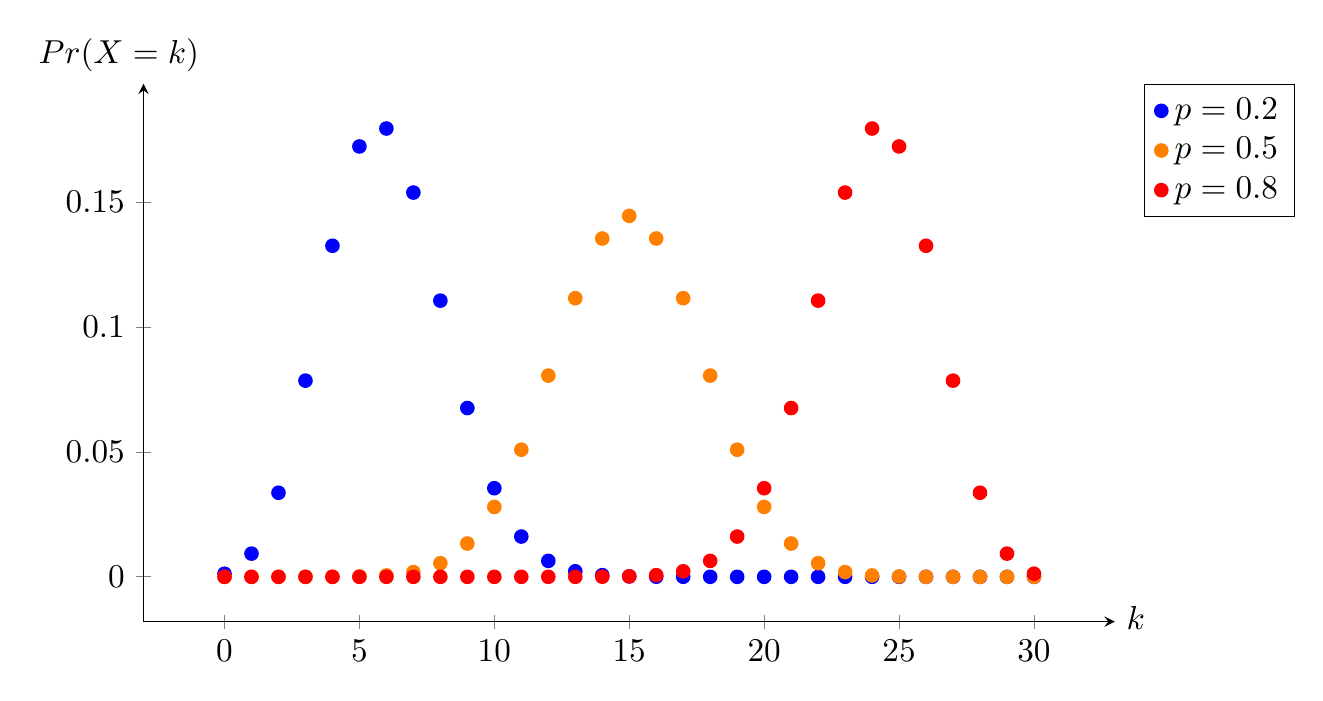
\begin{tikzpicture}[
        declare function = {binomial(\k,\n,\p)=\n!/(\k!*(\n-\k)!) * \p^\k * (1-\p)^(\n-\k);},
        scale = 1.2
    ]
        \begin{axis}[
            axis lines = left,
            enlargelimits = true,
            samples at = {0,...,30},
            xlabel = {$k$},
            ylabel = {$Pr(X=k)$},
            xlabel style = {at={(axis description cs:1,0.05)},anchor=north west},
            ylabel style = {at={(axis description cs:-0.12,1)},anchor=south west,rotate=-90},
            ytick = {0, 0.05, 0.1, 0.15},
            yticklabels = {0, 0.05, 0.1, 0.15},
            x post scale = 1.5,
            legend pos = outer north east,
            legend cell align = left,
        ]
            \addplot [only marks, blue] {binomial(x,30,0.2)};
            \addlegendentry{$p=0.2$}
            \addplot [only marks, orange] {binomial(x,30,0.5)};
            \addlegendentry{$p=0.5$}
            \addplot [only marks, red] {binomial(x,30,0.8)};
            \addlegendentry{$p=0.8$}
        \end{axis}
    \end{tikzpicture}
\end{figure}